%%%%%%%%%%%%%%%%%%%%%%%%%%%%%%%%%%%%%%%%%%%%%%%%%%%%%%%%%%%%%%%%%%%%%%%%
%                                                                      %
%     File: Thesis_StateofArt.tex                                      %
%     Tex Master: Thesis.tex                                           %
%                                                                      %
%     Author: Miguel Fonseca                                           %
%     Last modified : 17 August 2015                                   %
%                                                                      %
%%%%%%%%%%%%%%%%%%%%%%%%%%%%%%%%%%%%%%%%%%%%%%%%%%%%%%%%%%%%%%%%%%%%%%%%

\chapter{State-of-the-art}
\label{chapter:state}

\section{Unmanned Aircraft System}
\label{section:uas}
Multiple terms may be used when talking about unmanned aircraft. When referring to the aircraft \textit{per se}, one can use UA or UAV, which can be defined as "a reusable aircraft designed to operate without an onboard pilot which does not carry passengers and can be either remotely piloted or pre-programmed to fly autonomously." \citep{Angelov2012}. The FAA uses a different definition for UAs: "A device used or intended to be used for flight in the air that has no onboard pilot. This device excludes missiles, weapons, or exploding warheads, but includes all classes of airplanes, helicopters, airships, and powered-lift aircraft without an onboard pilot. UA do not include traditional balloons, rockets, tethered aircraft and un-powered gliders" \citep{FederalAviationAdministration2013}.\\
Unmanned Aircraft System includes all the systems that enable the operation of a UAV, which may include a ground control station and the communication links, among other things. It can be divided in three different segments \citep{Angelov2012}, as shown in figure \ref{fig:uas}: air segment (UAs and their payloads), ground segment (ground control station) and communications segment (Command and Control data link, Payload data link and External Communications).

\begin{figure}[!htb]
  \centering
  \includegraphics[width=0.5\textwidth]{Figures/UAS.png}
  \caption[Unmanned Aircraft System (UAS) Segments \citep{FederalAviationAdministration2013}]{UAS Segments: Air, Ground and Communications \citep{FederalAviationAdministration2013}}
  \label{fig:uas}
\end{figure}

Since the mechanical bird created by Archytas the Tarantine in 425 B.C., which is considered to be the first autonomous mechanism \citep{Angelov2012}, the evolution of unmanned vehicles was initially very slow. Only in 1916 an aircraft was created that was capable of automatic stabilization by the Americans Lawrence and Sperry. After that, with the fast advancements in technology, the USA's Air Force was able to develop the Ryan Model 147 series which were used for reconnaissance missions over China and other countries in the 1960s and 1970s \citep{Angelov2012}. The first RQ-1 Predators were used on operations in former Yugoslavia. It would later be equipped with Hellfire anti-tank missiles and operate in combat missions after the September 11 attacks.\\
On the civilian side, the National Aeronautics and Space Administration (NASA) developed the Environmental Research Aircraft and Sensor Technology (ERAST) project during the 1990s. The developed aircraft was able to fly at altitudes of up to 30.000 m during long periods to carry out environmental measurements. Since then, the prices of electronic components decreased, as well as their size and weight. With increasingly available and affordable equipment, so did the general public interest to operate UA. According to \citep{Karp2015}, "as many as one million sUA are expected to be sold during the 2015 US holiday season".\\
With the development of UA technologies, the already high number of possible applications for unmanned aircraft is only increasing. These can be grouped in different categories, such as \citep{Angelov2012}:
\begin{itemize}
\item Military applications (intelligence, surveillance, reconnaissance, strikes, etc...)
\item Environmental applications (remote environmental research, magnetic field measurement, etc...)
\item Emergency applications (firefighting, search and rescue, etc...)
\item Communications applications (telecommunication relay services, etc...)
\item Monitoring applications (crop and harvest, infrastructure, etc...)
\item Commercial applications (aerial photography, package delivery, etc...)
\end{itemize}
This increase in the number of operating UA with no existing regulations has also raised the concern of a higher collision risk. The amount of incidents reported has been rising: on September 21st, 2014, a helicopter pilot reported a near collision with a small unmanned aircraft vehicle above the Schuylkill County's Joe Zerbey Airport, Pennsylvania, USA \citep{Choate2014}; on August 30th, 2015, a light aircraft collided with what is believed to be an unmanned air vehicle without any resulting technical problems around Vasser, Norway \citep{Kaminski-Morrow2015}; during August 2015, four near-misses involving small unmanned aircraft took place near major UK airports, such as Heathrow \citep{Paton2015}.
\section{Sense and Avoid}
\label{section:saa}
\textbf{Sense and Avoid} (SAA) is the function that allows an autonomous vehicle to detect conflicts during flight and enables it to create solutions to resolve it \citep{Angelov2012}. For detecting hazards, it isn't necessary to identify them, just to determine an object presence and to evaluate if the object is a threat or not \citep{Elliott2012}. The hazards may be incoming air traffic such as aircraft, gliders or balloons, or terrain and other obstacles such as buildings.\\
On manned aircraft this task is performed by pilots and is called \textbf{see and avoid}. The pilots need to regularly scan visually the available field of view in order to detect hazards. The scans may be more focused in areas where hazards are expected, as informed by air traffic control (ATC) or by electronic equipment \citep{Angelov2012}. After detecting the object, the pilot will decide if a trajectory modification is required or not. The practice of see and avoid can be demanding in poor visibility conditions or due to high air traffic, among other reasons \citep{AustralianTransportSafetyBureau2004}.\\
Without a pilot on-board, there needs to be a replacement capable of observing the surrounding, detecting hazards and avoiding them. This replacement may be a system that depends on on-board, off-board or both types of sensors, and the decision making can also be off-board at a control station or done by the aircraft's own system \citep{Angelov2012}.\\
A Sense and Avoid system can provide two types of services \citep{Angelov2012}. The first one is a self-separation service, which provides earlier maneuvers in order to keep an intruder from entering the "remain-well-clear volume" \citep{ICAO2015}, as depicted in figure \ref{fig:separation}. The other service is collision avoidance, which relies on aggressive maneuvers to avert threats from entering a smaller separation zone, called collision volume \citep{ICAO2015}. The separation volumes required between UAS, especially sUA, need to be adjusted, due to their lower size and velocity \citep{Angelov2012}, which should not require such great distances.\\

\begin{figure}[!htb]
  \centering
  \includegraphics[width=0.7\textwidth]{Figures/separationzones.png}
  \caption[Separation volumes and limits \citep{ICAO2015}]{Separation volumes and limits \citep{ICAO2015}}
  \label{fig:separation}
\end{figure}

In order to provide this separation, a Sense and Avoid system may use cooperative and non-cooperative equipment. Cooperative systems rely on communications between the involved aircraft to enable both detection and resolution, and thus require both aircraft to be equipped with specific equipment to do so. On the other hand, non-cooperative systems must function independently from the intruder, which usually has some limitations, such as lower performance due to adverse weather conditions \citep{Angelov2012}.\\

\subsection{Evolution of See and Avoid}
\label{subsection:evolution}

At the start of the twentieth century, aviation took off with the Wright brothers' first flight. After that, many experimenters designed and built all sorts of aircraft. Most of these aircraft would crash regularly due to lack of scientific knowledge to build them which culminated in non-existing laws and regulations to certify the manufacture of aircraft \citep{Nolan2010}. Those frequent crashes made the general public afraid of aviation, leaving it as a pastime for experimenters during a period.\\ 
Meanwhile, the first recorded night flight happened on October 22nd, 1909, and lasted 42 minutes "under a bright moonlight" \citep{Fischer1998}. For this flight, pilots Wilbur Wright and Lt. Frederic E. Humphries didn't use any equipment to improve visibility. This kind of equipment would only be introduced in August 1910: during a night exhibition, the involved pilots used lights on the wingtips and automobile horns to warn each other of their presence \citep{Fischer1998}.\\
During World War I, armies started to bomb their enemies using the cover of the night. Due to the airplanes' short range, airfields had to be near the front line. To protect them from enemy bombardment, all lights remained turned off until an approaching aircraft was identified. To identify themselves, they used flare signals or a unique Morse identifier from an on-board light \citep{Fischer1998}.\\
Until the decade of 1930, it was deemed unnecessary to regulate air traffic and pilots used the practice of "see and be seen" to fly safely. To enable it, they would only fly with weather conditions that allowed them to see other aircraft in time to prevent collisions. These rules would evolve into what is now known as visual flight rules (VFR).\\
With the evolution in technology and procedures, aviation got to the point where it was reliable enough to keep regular services. This created an increase in the number of aircraft using the airspace and, at the same time, introduced a new danger: mid-air collision.\\
With the increase of air traffic, the concentration of airplanes near airfields became problematic. On days with good weather conditions, it was possible to see aircraft landing and taking off in every direction \citep{Nolan2010}. To reduce the risk of collision, some airports started to have an air traffic controller. The air traffic controller would stand on the airfield communicating with pilots. Using several colored flags, they would advise pilots with various information, like takeoff clearance \citep{Nolan2010}. It wasn't long before this system was replaced by light guns with colored lenses, using a code like the old one.\\
The introduction of artificial horizon and ground-based navigation aids increased the ability for aircraft to fly with bad weather. Adding to this, the differences in speed and size between old and new aircraft meant that keeping the separation distances between flights would become increasingly difficult.\\
Again, the issue was more evident near major airports. As the number of aircraft exceeded the air traffic control capabilities, people who lived close to these airports started to fear a collision over their houses. Due to their pressure,  most states in the USA started to create legislation restricting flight. It soon became "apparent that utter chaos would result in the aviation industry if every state enacted legislation (...)."  \citep{Nolan2010}.\\
In the United States of America, the solution for this problem came from Congress, with the creation of the Bureau of Air Commerce. This agency was responsible for licensing pilots, establishing airways and navigation aids, and providing separation between aircraft using their airways. 
Due to budget restrictions, the Bureau delegated on the major airlines the development and operation of multiple airway traffic control units (ATCUs) to provide the required separation.\\
To operate in controlled airways, pilots had to file an instrument flight plan to the ATCUs.  This flight plan included the type of aircraft, the departure and arrival airports and other flight-related information. With this information, air traffic controllers were able to check for conflicts between flights. If needed, they would make changes to the flight plans before and after the airplanes took off. This active control allowed pilots to fly during adverse weather conditions safely.\\
Although initially successful, the separation of aircraft operating in the ATCUs' airways was still handicapped due to the lack of standardized procedures \citep{Nolan2010}.\\
It started to become clear that the practice of "see and be seen" and the existing ATCUs were not enough to provide the required separation.  Because of this, the Radio Technical Commission for Aeronautics (RTCA) formed a team to attempt to plan the future of aviation. This team would be know as the RTCA's Special Committee 31 (SC-31). In their final report, they made recommendations for the Air Traffic Control System (ATCS), but avoided the development of unusual technical equipment and insisted that any additions to the ATCS should meet the following requirements \citep{Nolan2010}:
\begin{enumerate}
\item The new system should permit aircraft to be flown safely
\item It should improve the flow of air traffic
\item Any airborne equipment should be both simple and lightweight
\item Any new system should impose the smallest burden possible on the pilot or ground personnel
\item The installed equipment should require the least funding from either taxpayers, airlines or private pilots
\end{enumerate}

The SC-31 also recommended the introduction of several technologies such as: VHF Omnidirectional Range (VOR) and  Distance Measuring Equipment (DME) for navigation, Airport Surveillance Radar (ASR) and a lightweight transponder for detection and collision avoidance, and Instrument Landing System (ILS) and Precision Approach Radar (PAR) for airfield approaches.\\
Due to budget restrains related with war effort, the necessary funds to expand the air traffic control services were not obtained \citep{Nolan2010}, with few recommendations being introduced in the following years.\\
By the end of the decade of 1940, the ATCS was no longer able to handle the  traffic operating in the airways, due to the outdated procedures. The required separation between aircraft was still achieved by separating them in the distance equivalent to 10 minutes, which meant separations between 50 and 100 miles. Because of this, and to avoid delays, pilots would operate under VFR or IFR in uncontrolled airspace, hoping there was no other aircraft within their vicinity.\\
Because of this behavior, in June 30th, 1956, a Lockheed Super Constellation from Trans World Airlines (TWA) collided with an United Airlines' aircraft over the Grand Canyon. Both airplanes were operating outside controlled airspace to reduce the travel distance. The death of all passengers and flight crew would then start a national effort to modernize the ATCS \citep{Nolan2010}.\\
Before any major change was made to the ATCS, a United Airlines DC-8 collided with a TWA Super Constellation over New York City on December 16th, 1960. Both aircraft were on holding patterns waiting for clearance to land in different airports. The DC-8 pilots didn't inform the ATC of a navigation system malfunction, deviating from their course and entering the TWA's assigned holding pattern. During the investigation that followed, it was determined that, had the ATC been equipped with the ASR equipment recommended by the SC-31, the collision could have been avoided \citep{NationalTransportationSafetyBoard1962}.\\
During this time, investigation to develop a collision avoidance system had already started and the efforts included an emphasis on passive and non-cooperative systems \citep{FederalAviationAdministration2011}.\\
To invert the habit of making changes after incidents, the Federal Aviation Administration (FAA) created a task force known as Project Beacon. This task force was responsible for investigating the ATCS and make recommendations for its improvement, as did the SC-31.
After one year of investigation, the Project Beacon task force issued their results:
\begin{itemize}
\item The FAA had no clear overall direction for their development projects.
\item The research being made by the FAA was still based on the SC-31 recommendations.
\item The research being made was focused on technically advanced equipment and not to solve the more immediate problems.
\item The radar equipment being used needed to be improved.
\end{itemize}
And made several recommendations, among which:
\begin{itemize}
\item Installation of enough radar surveillance equipment to allow ATCs to continuously monitor aircraft from takeoff to landing.
\item Installation of secondary radar and transponders to allow identification and determination of altitude of each aircraft.
\end{itemize}

The selected system to help the controllers more immediately was the Secondary Surveillance Radar (SSR), also know as Air Traffic Control Radar Beacon System (ATCRBS) in the USA. It was based on the Identification Friend or Foe (IFF) used by the military. The IFF allowed a ground-based transmitter to interrogate a nearby airplane: if a transponder equipped aircraft didn't respond with the correct reply, it was considered an enemy \citep{Chang2000}.\\
This first version of the SSR used the same principle: an interrogation-based system with signals similar to those used by the IFF system. The interrogations would be transmitted from a rotating antenna, obtaining replies from every aircraft carrying SSR transponders within that antenna's beam. This system used two separate modes to obtain identity (Mode A) and altitude (Mode C), complementing the radar detection with this information.\\ 
Although this first version was a great improvement to the radar detection technology already in use, it would overload in areas with great concentrations of air traffic \citep{Chang2000}. The overloading was due to the replies given by multiple aircraft's transponders inside the interrogating antenna's beam, which would generate interference, rendering unpredictable results \citep{Nolan2010}.\\
Due to the system's limitations and FAA's budget cuts, by late 1960's, the air traffic control system was once more in chaos. Following two collisions in 1967, a new committee was formed to predict the future of air traffic control, the Air Traffic Control Advisory Committee (ATCAC). This committee recommended the upgrade of the SSR, the update of runway and air separation standards and the development of a collision avoidance system.\\
In the beginning of the 1970's, several manufacturers worked together to develop aircraft collision avoidance systems which were based on time/frequency techniques and interrogators. Despite successful testing, they concluded that this type of systems would not increase security. This was due to their high rate of false alarms in dense terminal areas and that every aircraft would have to be equipped with the same equipment \citep{FederalAviationAdministration2011}.\\
Later, in 1974, the MITRE Corporation proposed the Beacon-Based Collision Avoidance System (BCAS). BCAS was an on-board system which relied in the transponders already being used by the SSR, sending interrogation signals to any nearby aircraft, instead of a ground station. With the responses transmitted by the intruder's transponder, BCAS could determine the location, speed and course of each airplane to help avoid collisions, independently from the ground air traffic control systems.\\
Because it used a system similar to SSR, BCAS had the same deficiencies \citep{Garr1979}: interference generated when multiple airplanes were inside the antenna's interrogation beam; couldn't detect aircraft above itself, as the SSR's antennas were positioned beneath the fuselage, shielding the signal; and could only give commands for vertical maneuvers, due to problems with the airborne antenna in providing accurate directional information.

The solution found for both the collision avoidance system and the air traffic control system was to upgrade the SSR, as recommended by the ATCAC. The upgrade consisted in using discrete addressing to reduce the amount of messages on the communication channels. Discrete addressing means that only the inquired aircraft will reply, instead of all aircraft inside the interrogating antenna's beam.
From this, manufacturers developed Mode S (for Select) system. It was designed to completely integrate with the ATCS, as one of the main concerns of the ATCAC was that aircraft owners would not be able to easily replace the old transponders, due to high manpower and parts costs as well as due to the long time required for the complete upgrade of all equipment. Because of this, the new system would have to be inter-operable with older Mode A/C \citep{Chang2000}, as shown in figure \ref{fig:modesinter}.\\

\begin{figure}[!htb]
  \centering
  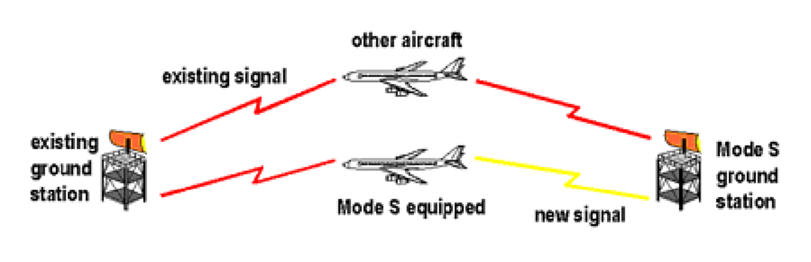
\includegraphics[width=0.80\textwidth]{Figures/modes.png}
  \caption[Interoperability: SSR and Mode S \citep{Chang2000}]{Interoperability: SSR and Mode S \citep{Chang2000}}
  \label{fig:modesinter}
\end{figure}

To use discrete addressing, each airplane has a unique identification code which is present in interrogations targeted for that airplane. Messages with a different identification code are ignored, only replying when the codes match.\\
Although the technology for Mode S was ready to use in 1975, it was not adopted immediately due to problems with manufacturing companies, which insisted in changing the initial design that made it malfunction or lack desired functions \citep{Chang2000}.\\
In 1978, a Pacific Southwest Airlines Boeing 727 collided with a private Cessna 172 during approach to Lindbergh Field in San Diego, California. The accident report states that, although the San Diego Approach Control had the capability to provide either vertical or lateral separation between IFR aircraft and participating VFR aircraft, the controller chose to give PSA 727 a visual separation clearance. This clearance gives the pilot exclusive responsibility of staying clear of other aircraft. Although the PSA pilots lost sight of the intruder Cessna, they trusted that the controller was still helping them maintaining separation and did not take timely measures to evade the aircraft which was now directly in front and below them. The following collision over a residential area resulted in the death of 137 people \citep{NationalTransportationSafetyBoard}.\\
%------TCAS------%
After this accident, the FAA increased the efforts to complete the development of an effective on-board collision avoidance system \citep{FederalAviationAdministration2011}. In 1981, FAA modified the BCAS design and created the Traffic Alert and Collision Avoidance System (TCAS), known as Airborne Collision Avoidance System (ACAS) outside the USA.\\
TCAS is an instrument integrated into other systems inside an aircraft cockpit. It is independent of the ATC ground systems, interrogating nearby ICAO compliant transponders \citep{Chang2000}. The reply contains information about range, bearing and altitude data which is used to predict collisions, prompting pilots to start evasive maneuvers \citep{FederalAviationAdministration2011}. With this, TCAS is able to help pilots with see and avoid: "TCAS functions as "electronic eyes" for pilots, providing them with an enhanced view of nearby flight traffic" \citep{MariaS.Lee2009}. \\
TCAS has two levels of sophistication: TCAS I and II. The simpler and more inexpensive TCAS I only alerts the pilot when other aircraft are close. TCAS II also provides resolutions advisories \citep{NationalTransportationSafetyBoard1986}.\\
In order to minimize the frequency of false alarms, the development of TCAS' algorithms meant the completion of several computer simulations, pilot in the loop simulations as well as testing prototype equipment on-board FAA aircraft \citep{FederalAviationAdministration2011}, which took several years to complete.\\

Meanwhile, in 1986, another mid-air collision forces changes in aviation. An Aerom\'{e}xico DC-9 collided with a private Piper PA-28-181 Archer, while approaching Los Angeles International Airport. The accident killed everybody on-board both aircraft and 15 people on the ground. During investigation, it was found that the Piper entered the Los Angeles Terminal Control Area airspace without the required clearance and that it was only equipped with a Mode-A transponder, which prevented the ATC from seeing its altitude \citep{NationalTransportationSafetyBoard1986}. Even so, both aircraft were flying in visual flight conditions and were responsible to see and avoid each other, which neither did.\\
Following this accident, the USA Congress passed the Airport and Airway Safety and Capacity Expansion Act in 1987, requiring that all carrier aircraft operating within US airspace with more than 30 passenger seats would have to be equipped with TCAS II by 1993. Aircraft with 10 to 30 seats were only required to be equipped with TCAS I \citep{SenateandHouseofRepresentativesoftheUnitedStatesofAmericainCongress1987}.\\
In Europe, EUROCONTROL defined the beginning of the year 2000 as the limit for all civil fixed-wing turbine-powered aircraft with a maximum take-off mass exceeding 15000 kg, or a maximum number of passengers of more than 30, to be equipped with TCAS II Version 7.0 and January 1st, 2005, for all civil fixed-wing, turbine-powered aircraft having a maximum take-off mass exceeding 5700 kg, or a maximum number of passengers of more than 19, to be equipped with TCAS II, Version 7.0 \citep{FederalAviationAdministration2011}.\\
ICAO would later require the implementation of TCAS II from January 1st, 2003 for all turbine-engine airplanes with a maximum take-off mass exceeding 15000 kg, or a maximum number of passengers of more than 30, and from 1 January 2005 for aircraft with more than 5700 kg or 19 passengers. ICAO also recommends that all aircraft should be equipped with a TCAS II \citep{Icao2006}.\\
%------ADS-B------%
In 1996, to avoid FAA expenditures in operating, maintaining and replenishing the old radar surveillance infrastructure, the FAA published the Surveillance Vision Plan (SVP). The SVP describes the FAA's next aircraft surveillance system, presenting a plan for its implementation in 5-year segments through 2015. It "describes the transition from ground-based radar surveillance to a joint satellite-based and ground-based surveillance system" \citep{FAA1996}.\\
The cornerstone for the new aircraft surveillance system is a collaborative system, the Automatic Dependent Surveillance-Broadcast (ADS-B). ADS-B is a technique where the aircraft position is obtained by an on-board global navigation satellite system (GNSS) receiver and then its identity, altitude and position are broadcast directly to the ground and nearby aircraft, without using satellites. It is a system similar to TCAS but ADS-B extends the same techniques to ground-based surveillance over great ranges.\\
In the USA, aircraft will only be required to operate with ADS-B after January 1st, 2020. Until then, the FAA is broadcasting traffic, weather and aeronautical information to already equipped aircraft at no cost, to motivate aircraft owners to update their systems \citep{FederalAviationAdministration2015a}.\\
In Europe, all aircraft with maximum take-off mass greater than 5700 kg or maximum cruising True Air Speed greater than 250 kts have to be equipped with ADS-B, after 8 June 2016 for forward fit and June 7th, 2020, for retrofit \citep{TheEuropeanCommission2014} \: \citep{TheEuropeanCommission2011}.

\subsection{See and Avoid in General Aviation}
\label{subsection:gat}
In the general aviation, there are several technologies that complement the practice of see and avoid. The most important are discussed bellow.

\subsubsection{Position and Anti-Collision Lights}
\label{subsubsection:poslights}
One of the first systems created to help see and avoid were the Position Lights. 
Based on the system used in maritime navigation, it evolved into what is used today, showed in \ref{fig:navlights1}.

\begin{figure}[!htb]
  \centering
  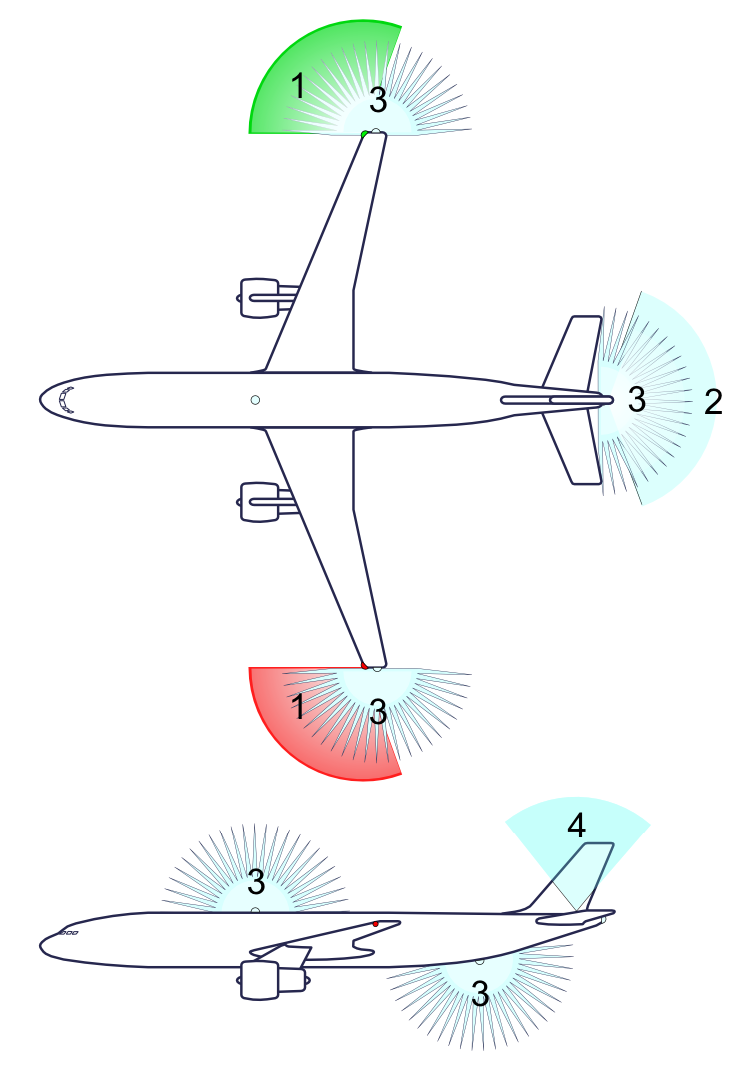
\includegraphics[width=0.35\textwidth]{Figures/navigationlights.png}
  \caption[Aviation Lights used in See and Avoid \citep{Tosaka2010}]{Aviation Lights used in See and Avoid. 1) Left and Right Position Lights; 2) Rear Position Light; 3) Anti-collision Lights; 4) Logo Light; \citep{Tosaka2010}}
  \label{fig:navlights1}
\end{figure}

The position lights must be turned on from sunset to sunrise for aircraft operated on the surface and in flight. The Anti-Collision lights must be on during all operations, day or night, except when they may constitute a hazard to safety during adverse meteorological conditions \citep{FederalAviationAdministration2015a}.\\
The position lights system must be composed by a red light on the left side and a green light on the right side, spaced as far as practicable, and a white light mounted as far back as possible (on the tail or each wing tip) \citep{Easa2012}.
The left (L) and right (R) position lights' dihedral angles are formed by two intersecting vertical planes, one parallel to the longitudinal axis of the aircraft and a second at 110\degree to the left and the right, respectively, as viewed when looking from the back to the front of the airplane \citep{Easa2012}. 
The rear (A) position light dihedral angle is formed by two intersecting vertical planes, each making a 70\degree angle to the right and to the left to a vertical plane parallel to the longitudinal axis \citep{Easa2012}. \\
In the horizontal plane, the position lights have the intensity requirements in \ref{tab:inthor}. For any vertical planes, the requirements depend on the horizontal plane minimum intensity I, and gradually decrease until a minimum is reached at 90\degree .\\

\begin{table}[!htb]
\begin{center}
\caption[Minimum intensities in the horizontal plane for position lights \citep{Easa2012}]{Minimum intensities in the horizontal plane for position lights \citep{Easa2012}.}
\begin{tabular}{ccccc}
Light Position & \multicolumn{3}{c}{Left and Right} & Rear \\ 
\hline 
Angle measured from dead ahead & 0\degree to 10\degree & 10\degree to 20\degree & 20\degree to 110\degree & 110\degree to 180\degree \\ 
Intensity (candelas) & 40 & 30 & 5 & 20 \\ 
\end{tabular}
\end{center}
\label{tab:inthor}
\end{table}

The position lights also have maximum intensities in overlapping beams of position lights \citep{Easa2012}.\\

For the anti-collision light system, an aircraft must have one or more approved aviation red or aviation white anti-collision lights located in a place that will not diminish the pilot's vision and the position lights visibility. These lights must have a field of coverage greater than or equal to 75\degree bellow and above the horizontal plane with no more than 0.5 steradians of obstructed visibility \citep{Easa2012}. They should also have a flash frequency between 40 and 100 cycles per minute, and between 40 and 180 in any overlaps when the system has more than one light.
Each anti-collision light must have an effective intensity which depend on the duration of the blink \citep{Easa2012}.

\subsubsection{Mode S}
\label{subsubsection:modes}

Mode S was designed to solve several faults in the previous Modes A and C. 

While addressing the problems with interference generated with the increasing amount of replies in the communication channels already approached in \ref{subsection:evolution}, mode S was designed as a discrete addressing system. This means that each aircraft's transponder has a unique identification code and will not answer to interrogations containing a different one.

As discussed in section \ref{subsection:evolution}, one of the requirements for Mode S was the interoperability with older modes, which meant that the new technology must be retro-compatible and transparent. \\
In order to achieve retro-compatibility, the same frequencies (1030 MHz uplink and 1090 MHz downlink) are used in Mode S. This allows new Mode S equipment to receive and interpret signals from SSR. On the other hand, the use of the same frequencies makes it harder for the new Mode S signal not to interfere with previous system's transponders and ground stations (transparency). This problem was solved using the sidelobe suppression technique used in the SSR which consisted in the comparison of two pulses P1 and P2 \citep{Chang2000}. SSR equipment was able to compare the signal (P1) from the main directional antenna with the signal (P2) transmitted by an omnidirectional antenna immediately after P1. P2 is weaker in the direction of the main lobe of P1, but stronger otherwise, as can be seen in figure \ref{fig:suppression}. If an aircraft was located inside P1 main lobe, like aircraft 1, it would receive a much stronger P1 pulse than P2, and a stronger P2 otherwise, as can be seen in figure \ref{fig:suppressionpulses}. SSR transponders only answer in positions where P1 pulse is stronger than P2, like aircraft 1. When located in other places, the transponder would be temporarily disabled for 35 microseconds \citep{Chang2000}.

\begin{figure}[!htb]
  \centering
  \includegraphics[width=0.35\textwidth]{Figures/suppression.png}
  \caption[ATCRBS Broadcast with Omnidirectional Antenna \citep{Chang2000}]{ATCRBS Broadcast with Omnidirectional Antenna \citep{Chang2000}}
  \label{fig:suppression}
\end{figure}

\begin{figure}[!htb]
  \centering
  \includegraphics[width=0.35\textwidth]{Figures/suppressionpulses.png}
  \caption[ATCRBS Broadcast Pulses \citep{Chang2000}]{ATCRBS Broadcast Pulses (A1 - aircraft 1; A2 - aircraft 2) \citep{Chang2000}}
  \label{fig:suppressionpulses}
\end{figure}

To enable transparent operation, mode S was designed to use this technique: its signal begins with two pulses similar to the one received by an aircraft on the sidelobe of an SSR ground station. After receiving this signal, SSR equipment will be disabled for 35 microseconds and only mode S equipment will receive the remaining signal.\\
The shape of mode S signal can be seen in figure \ref{fig:suppressionmodes}. Because mode S can only transmit while SSR equipment is disabled, the transmitted message was restricted to a length of 112 bits \citep{Chang2000}.\\

\begin{figure}[!htb]
  \centering
  \includegraphics[width=0.50\textwidth]{Figures/suppressionmodes.png}
  \caption[Mode S Signal with Sidelobe Suppression \citep{Chang2000}]{Mode S Signal with Sidelobe Suppression \citep{Chang2000}}
  \label{fig:suppressionmodes}
\end{figure}

Mode S introduced "the technical base for a digital communication exchange system" \citep{OfficeofTechnologyAssessment1980}. This capacity would bring an increase in the development of several services that, using the digital link, would be inexpensive to implement and use, like the Traffic Information Service, the Graphical Weather Service and TCAS.

\subsubsection{ACAS}
\label{subsubsection:tcas}
The Airborne Collision Avoidance System (ACAS) was introduced to reduce the risk of mid-air collisions, by providing pilots advice through resolution advisories (RAs) and traffic advisories (TAs). RAs are maneuvers recommended to the pilot to avoid an intruder aircraft, while TAs help the pilot visually acquire the position of the intruder.\\
ACAS was designed as a back-up for the ATC system and is not dependent on ground-based systems \citep{Icao2006}. By interrogating Mode A/C and Mode S transponders on nearby aircraft and processing their replies, ACAS is able to determine potential collision threats and provide the appropriate advisories to avoid them \citep{Eurocontrol2010}, with three different levels of capability:
\begin{itemize}
\item ACAS I provides information to aid "see and avoid" and does not provide RAs. It is usually installed on rotorcraft and small fixed-wing aircraft \citep{Icao2006}.
\item ACAS II provides TAs and RAs with vertical maneuvers to increase or maintain the vertical separation from an intruder aircraft. It was designed to be installed on fixed-wing aircraft \citep{Icao2006}. 
\item ACAS III is a system that provides RAs using vertical and horizontal maneuvers to increase or maintain the existing separation. There are no ACAS III implementations to date \citep{Eurocontrol2010}.\\
\end{itemize}
As an implementation of ACAS III is not expected due to difficulties with horizontal tracking \citep{Eurocontrol2015}, there is research being conducted to develop the next version of ACAS, ACAS X, which will use dynamic programming to optimize the generation of RAs \citep{Eurocontrol2015}.
As the only fully compliant implementation of ACAS I and II, to date, is the Traffic alert and Collision Avoidance System (TCAS) I and II, respectively, the terms ACAS and TCAS can be used interchangeably \citep{Eurocontrol2015}.\\
The level of protection given by TCAS depends on the equipment inside the target aircraft, as can be seen in table \ref{tab:tcasprotec}. If the target aircraft does not have an operating transponder, TCAS cannot provide any protection \citep{FederalAviationAdministration2011}.\\

\begin{table}[!htb]
\begin{center}
\caption[TCAS Levels of Protection \citep{FederalAviationAdministration2011}]{TCAS Levels of Protection \citep{FederalAviationAdministration2011}.}
\begin{tabular}{cccc}
                                           &                      & \multicolumn{2}{|c}{Own Aircraft Equipment}                  \\
                                           & \multicolumn{1}{l}{} & \multicolumn{1}{|c}{TCAS I} & \multicolumn{1}{c}{TCAS II}    \\ \hline
\multirow{4}{*}{Target Aircraft Equipment} & \multicolumn{1}{c|}{Mode A}              & TA                         & TA                             \\
                                           & \multicolumn{1}{c|}{Mode C or Mode S}    & TA                         & TA and Vertical RA             \\
                                           & \multicolumn{1}{c|}{TCAS I}              & TA                         & TA and Vertical RA             \\
                                           & \multicolumn{1}{c|}{TCAS II}             & TA                         & TA and Coordinated Vertical RA \\ \hline
\end{tabular}
\end{center}
\label{tab:tcasprotec}
\end{table}

When a target aircraft is in range and after several consecutive replies received from its transponder, TCAS divides the range with the closure rate, calculating the time, also known as \textit{tau}, until the Closest Point of Approach (CPA). After this, depending on the type of TCAS, it can issue the already mentioned TAs and RAs. Traffic Advisories will always be issued first, to help the pilot detect the target or to prepare him for an RA (only in TCAS II), when the \textit{tau} is bellow 20 or 48 seconds (with own altitude $<$1000 ft or $>$42000 ft respectively). If the aircraft is equipped with TCAS II, an RA will be issued, when the \textit{tau} is bellow 15 seconds for an altitude between 1000 ft and 2350 ft, and 35 seconds for an altitude greater than 42000 ft, containing recommended maneuvers. The \textit{tau} defines the protection volume given by TCAS, as shown in figure \ref{fig:tcasvolume}. If the target aircraft is also equipped with TCAS II, the RAs will be automatically coordinated through Mode S communications \citep{FederalAviationAdministration2011}.\\

\begin{figure}[!htb]
  \centering
  \includegraphics[width=0.90\textwidth]{Figures/tcasvolume.png}
  \caption[TCAS Protection Volume \citep{FederalAviationAdministration2011}]{TCAS Protection Volume - Not to scale \citep{FederalAviationAdministration2011}}
  \label{fig:tcasvolume}
\end{figure}

In order to have a fully functional TCAS II, an aircraft needs to have several components, as shown in figure \ref{fig:tcashardware}.\\

\begin{figure}[!htb]
  \centering
  \includegraphics[width=0.90\textwidth]{Figures/TCAShardware.png}
  \caption[Block diagram of TCAS and transponder hardware components required for standard TCAS equipment \citep{QinetiQ2013}]{Block diagram of TCAS and transponder hardware components required for standard TCAS equipment \citep{QinetiQ2013}}
  \label{fig:tcashardware}
\end{figure}

The TCAS II Processor uses data from several sensors, like radar altimeter, to monitor the aircraft state. At the same time, it performs airspace surveillance and intruder tracking simultaneously, using the Mode S Transponder to coordinate complementary RAs, when required, via the provided air-to-air data exchange protocol already mentioned in chapter \ref{subsubsection:modes}.
The TCAS and SSR control panel is the platform that allows the flight crew to control all TCAS equipment, including the Mode S transponder. It usually provides four different control positions \citep{FederalAviationAdministration2011}: 
\begin{itemize}
\item Standby - TCAS does not issue interrogations, Mode S Transponder replies only to discrete interrogations.
\item Transponder - Mode S Transponder operational, replying to all appropriate ground and TCAS interrogations. TCAS in standby.
\item TA Only - Mode S Transponder operational. TCAS operational but will only issue TAs.
\item Automatic - Mode S Transponder operational. TCAS operational, issuing the appropriate TAs and RAs.
\end{itemize}

In order to provide airspace surveillance and track intruders, TCAS needs several antennas, including a top directional antenna and a bottom antenna.  The antennas transmit interrogations at 1030 MHz and receive replies at 1090 MHz. The system may share these antennas with the Mode S transponder or have separate ones \citep{FederalAviationAdministration2011}.\\
Finally, the system uses both visual and aural signals to present the information to the flight crew, using predefined symbols and words.\\

Although TCAS is being tested for UAS use, it cannot be directly installed on an unmanned aircraft, as it was not designed for that purpose \citep{Icao2006}, but only for aircraft with an on-board pilot which is responsible for evaluating all the available information and decide to follow the RA or not. Adding to this, TCAS II was developed for fixed-wing aircraft and not for the different configurations available for unmanned aircraft which present different performance spectrum that may be outside the one required for response times, vertical accelerations and vertical rates in TCAS II \citep{Eurocontrol2010}.
Due to the amount of required equipment, TCAS is nowadays too large, heavy, power consuming \citep{Elliott2012} \citep{FederalAviationAdministration2015} and prohibitively expansive for small UAS operations, with the TCAS I equipment price above \$ 25,000 \citep{Smith2005}. Finally, TCAS can only reliably provide surveillance with traffic densities lower than or equal to 0.3 aircraft per square nautical mile (24 aircraft within 5 nmi radius) \citep{FederalAviationAdministration2011}, which may not be enough for the desired operation.
 

\subsubsection{ADS-B}
\label{subsubsection:adsb}

As mentioned in \ref{subsection:evolution}, the Automatic Dependent Surveillance-Broadcast (ADS-B) is a technique that, using the position obtained by an on-board GNSS receiver, broadcasts (ADS-B Out) the aircraft's state vector (3D position and 3D velocity) for ground-based and aircraft-based surveillance \citep{Lester2007} \citep{Costin2012}, as can be seen in figure \ref{fig:adsbscheme}.

\begin{figure}[!htb]
  \centering
  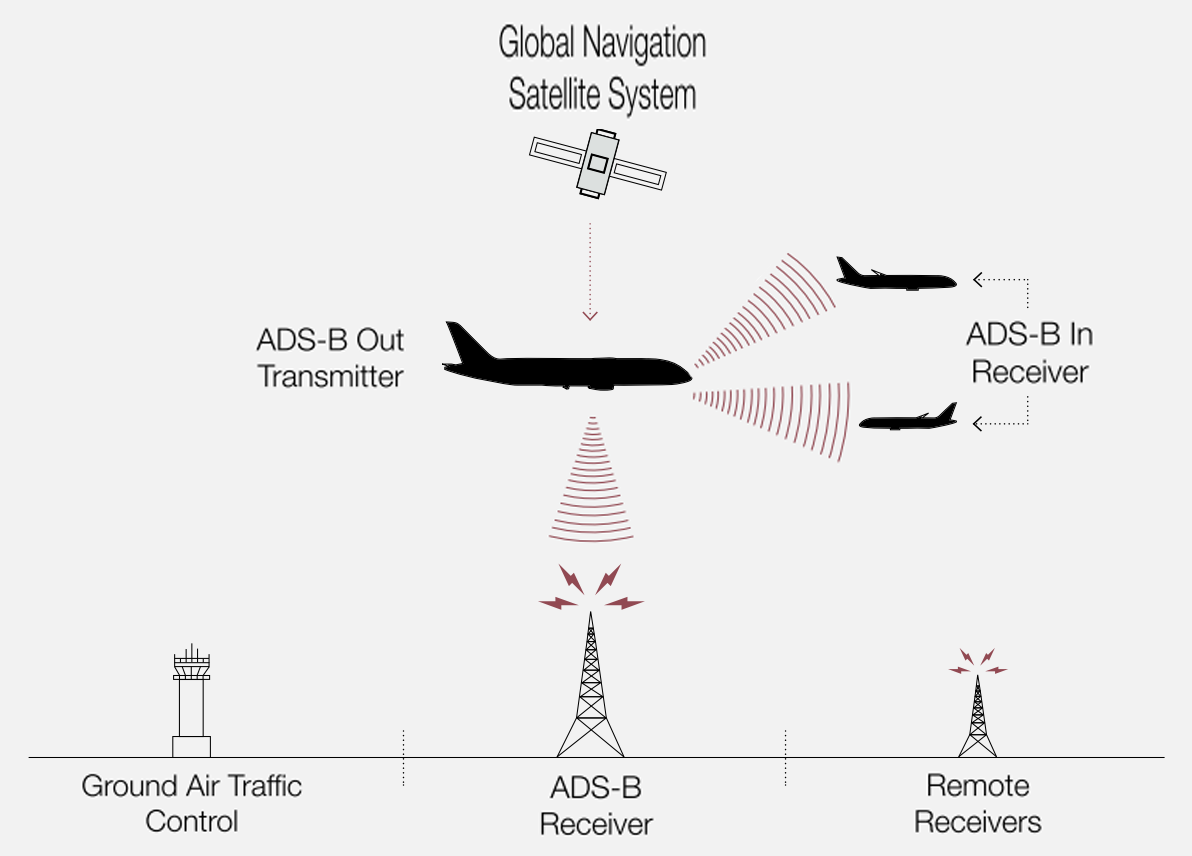
\includegraphics[width=0.90\textwidth]{Figures/ADS-B2.png}%ADS-B1.jpg}
  \caption[ADS-B communications \citep{Richards2010}]{ADS-B communications \citep{Richards2010}}%%\citep{Allen2012}}
  \label{fig:adsbscheme}
\end{figure}

By providing this information to nearby aircraft (ADS-B In), the pilots can perform collision avoidance without instructions from the ATC \citep{Lester2007} \citep{Costin2012}. With the received state vector and its own, the aircraft is able to calculate relative range and bearing to the transmitting aircraft and display this information to the pilot on a Cockpit Display of Traffic Information (CDTI). 

ADS-B, as a broadcast technology, does not require any replies. The aircraft is always broadcasting it's state vector unlike TCAS, which only sends information when interrogated. Since it does not require any action from the pilot, it is automatic. Finally, as it depends on the aircraft to acquire its position and its transmitter to broadcast the signal, it is considered as dependent surveillance.

There are several data links to enable ADS-B communication: Mode S 1090 MHz Extended Squitter (1090-ES), Universal Access Transceiver (UAT) operating at 978MHz and VDL (VHF Digital Link) Mode 4. The FAA has only approved the first two, while EUROCONTROL only accepts 1090-ES.

1090-ES is an update to Mode S, mentioned in subsection \ref{subsubsection:modes}.  When equipped with this version of Mode S transponder, an aircraft transmits the additional data required for ADS-B Out, without interrogations from TCAS or SSRs.

UAT is a data link used for wideband broadcast operating on 978MHz that has a modulation rate of 1.042 Mbps \citep{ACP2005}. It was designed for ADS-B communications but it also supports other related services, like Flight Information Service - Broadcast (FIS-B) and Traffic Information Service - Broadcast (TIS-B). Although it was initially thought to be the most probable protocol to be adopted for ADS-B, it hasn't been accepted internationally because it operates in frequencies close to some DME stations \citep{Lester2007}.  

Finally, VDL Mode 4 is a protocol designed by a Russian-Swedish cooperation. It operates in 108-137 MHz range, using 25kHz communication channels and has a modulation rate of 0.0315 Mbps with a D8PSK modulation scheme or 0.0192 Mbps with a Gaussian-filtered Frequency Shift Keying \citep{proesch2015}. It supports both communications data link and surveillance data link. It was rejected in the USA due to its high implementation cost as well as the lack of ICAO assigned frequencies at the time \citep{Lester2007}.

Although the ADS-B out technology offers a better solution for collision avoidance than TCAS, the upgrade may have high costs for operators. Depending on the required ADS-B standard, the operator may have to upgrade to a wide area augmentation system (WAAS) certified GNSS receiver and/or a new flight management system (FMS) computer \citep{Lester2007}.

\section{New developments on SAA}
\label{section:newsaa}
With the increase of UA use, the problem of operations in the same airspace as manned aircraft has to be dealt with.
There are already several proposals and guides to regulate this problem, but only some countries have defined requirements and laws that regulate UA's use.\\
In Europe, although EUROCONTROL has published no legislation for UA under 150 kg, several European countries have their own requirements. The United Kingdom released on 29 May 2002 the Civil Aviation Publication 722 - Unmanned Aircraft System Operations in UK Airspace - Guidance, which was last updated on 24 March 2015. This document provides guidance for UK unmanned aircraft users.\\
In the United States of America, the FAA has proposed regulation for Unmanned Aircraft Systems on the first trimester of the year 2015.\\
Until now, all the existing legislation is only allowing operations in segregated airspace due to, as mentioned in \ref{section:saa}, the impossibility of using see and avoid without a pilot on-board. In order to enable operations in non-segregated airspace, an SAA solution that can provide the required separation must be created \citep{FederalAviationAdministration2015}.\\
Multiple authorities state that UA must provide at least the same reliability as manned aircraft to operate in the same airspace \citep{InternationalCivilAviationOrganization2011}. In order to achieve the required reliability, UA would have to use high reliability components or increase hardware redundancy \citep{Angelov2012}, like the general aviation. Due to limits in sUA payload dimensions and weight as well as the cost benefit of the activities where sUA may be involved, both options may not be easy to implement: higher reliability components are more expensive than the equipment being used now and it is almost impossible to increase the hardware redundancy without exceeding the aircraft maximum payload. These limitations create a problem with the kind of payload that might be used for SAA.\\
As mentioned in section \ref{subsubsection:tcas}, TCAS and ADS-B both require equipment that is not appropriate for sUA \citep{FederalAviationAdministration2015}. Although ADS-B's use in GA is growing, the required (certified) GNSS equipment represents a cost that most sUA users cannot afford. By using non-certified equipment, the obtained position has a much higher position error and there is no error estimation provided. Adding to this, the required transmitting equipment for both ADS-B and TCAS is still too large, heavy and power consuming for an appropriate range.\\
A possible solution is to lower the requirements for small UA's SAA reliability proportionally to their size, weight and velocity.\\
Another step to enable UA operations in unsegregated airspace, is to develop and mandate a short-range, low power and lightweight cooperative technology for collision avoidance first and a non-cooperative later, as the development of a technology that enables the detection of non-cooperative aircraft may cost US\$ 2 billion and take several more years \citep{Angelov2012}.\\

\section{SAA development programs}
\label{section:saaprograms}
Due to the increasing availability and disseminated use of UA, the risk of a collision is increasing. In an attempt to prevent this, there are already several programs worldwide studying sense and avoid. Some of them are presented bellow.\\
\subsection{MIDCAS}
The Mid Air Collision Avoidance System Project is an european industrial consortium composed by: SAAB, Alenia Aeronautica, CIRA (Italian Aerospace Research Center), Diehl BGT Defence, DLR (German Aerospace Center), Airbus Defense and Space, ESG Elektroniksystem- und Logistik-GmbH, Indra, Sagem, Selex ES and Thales. It was launched in 2009 by five member states (France, Germany, Italy, Spain and Sweden) under the framework of the European Defence Agency with three main focus \citep{Consortium2011}:
\begin{itemize}
\item Progress on Standards for SAA.
\item Design of a generic SAA function to be tested in simulations.
\item Design of an SAA Demonstrator to be tested in manned and Remotely Piloted Aircraft Systems (RPAS) flight.
\end{itemize}
Their aim is to contribute to the RPAS integration in civilian airspace by proposing a baseline of solutions for the "Unmanned Aircraft System Mid-air Collision Avoidance Function" acceptable by the manned aviation.\\
Flights tests with Alenia Aeronautica's Sky-Y with a payload of SAA cooperative and non-cooperative sensors, as can be seen in figure \ref{fig:midcas}, were performed in Italy between December 2014 and April 2015. During this time, the UA was able to perform fully automated avoidance maneuvers to avoid collision with a manned aircraft.

\begin{figure}[!htb]
  \centering
  \includegraphics[width=0.90\textwidth]{Figures/midcas.jpg}
  \caption[Sense and Avoid Demonstrator \citep{EuropeanDefenceAgency2015}]{Sense and Avoid Demonstrator \citep{EuropeanDefenceAgency2015}}
  \label{fig:midcas}
\end{figure}
	
\subsection{UAS Integration in the NAS Project}
The UAS Integration in the National Airspace System (NAS) Project is the FAA's attempt to integrate unmanned aircraft into the NAS "without reducing existing capacity, decreasing safety, negatively impacting current operators, or increasing the risk to airspace users or persons and property on the ground any more than the integration of comparable new and novel technologies" \citep{FederalAviationAdministration2013}.
Its goal is to reduce technical barriers associated with integrating UAS into the NAS utilizing integrated system level tests in a relevant environment \citep{Rugg2015}.\\
In 2013, the project published the Integration of Civil Unmanned Aircraft Systems (UAS) in the NAS Roadmap, with the purpose of outlining, "within a broad timeline, the tasks and considerations needed to enable UAS integration into the National Airspace System (NAS) for the planning purposes of the broader UAS community" \citep{FederalAviationAdministration2013}. This roadmap defines a 5 year near term, 5 to 10 mid-term and a longer than 10 years long-term with plans and expected results for each period. All three terms try to harmonize with the international community and several segments of society (industry, civil liberties and national security), namely with ICAO, following the considerations on the Circular 328 "Unmanned Aircraft Systems (UAS) Circular". This circular provides guidelines for Member States to integrate UAS into their airspace in a consistent manner, so that global compatibility may be achieved when possible.\\
%To help the FAA in the integration of the UAS in the NAS, the RTCA formed the Special Committee 203 (SC-203) in 2004. The SC-203 developed and published several guidelines for UAS integration \citep{FederalAviationAdministration2013}:
%\begin{itemize}
%\item UAS must operate safely, efficiently, and compatibly with service providers and other users of the NAS so that overall safety is not degraded;
%\item UAS will have access to the NAS, provided they have appropriate equipage and the ability to meet the requirements for flying in various classes of airspace;
%\item Routine UAS operations will not require the creation of new special use airspace, or modification of existing special use airspace;
%\item Except for some special cases, such as small UAS (sUAS) with very limited operational range, all UAS will require design and airworthiness certification to fly civil operations in the NAS;
%\item UAS pilots will require certification, though some of the requirements may differ from manned aviation;
%\item UAS will comply with ATC instructions, clearances, and procedures when receiving air traffic services; 
%\item UAS pilots (the pilot-in-command) will always have responsibility for the unmanned aircraft while it is operating;
%\item And UAS commercial operations will need to apply the operational control concept as appropriate for the type of operation, but with different functions applicable to UAS operations.
%\end{itemize}
%Meanwhile, the FAA has established several UAS test sites to help them gain a better understanding of operational issues. Although privacy policies are not part of the FAA mission, any one operating at these test sites will have to develop a privacy policy. The developed privacy policies will help "inform the dialogue among policymakers, privacy advocates, and the industry regarding broader questions concerning the use of UAS technologies in the NAS" \citep{FederalAviationAdministration2013}.\\

\subsection{Geyer's prototype SAA system}
Carnegie Melon University's investigators approached SAA using vision systems, avoiding cooperative communication systems \citep{Geyer2008} \citep{Geyer2009} \citep{Dey2010}. To determine the minimum requirements of the sense component, they first developed the collision avoidance component and computed its maximum performance.\\
Their work was divided into the following tasks \citep{Geyer2009}:
\begin{itemize}
\item Task 1: develop an aircraft detection and collision warning system prototype.
\item Task 2: develop a collision avoidance system prototype.
\item Task 3: investigate alternative technologies.
\end{itemize}

It was found that the performance factors for an SAA system that uses vision can either be controllable or not, as showed in figure \ref{fig:geyer1}.
\begin{figure}[!htb]
  \centering
  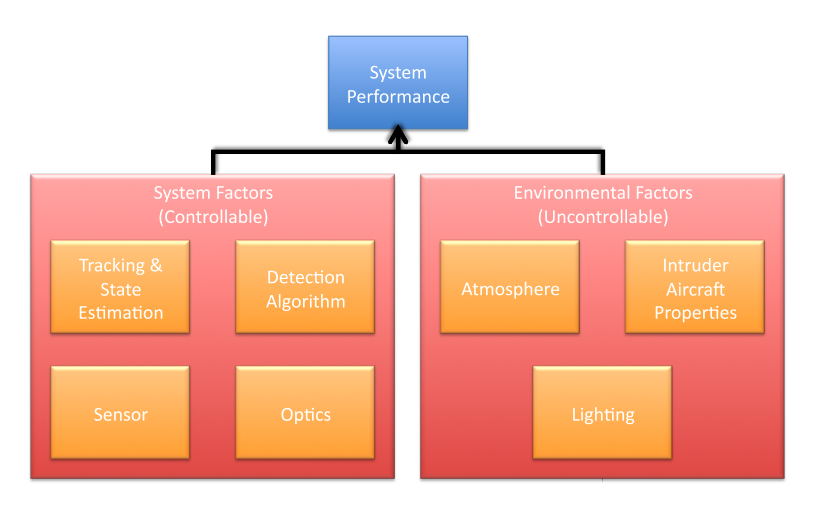
\includegraphics[width=0.90\textwidth]{Figures/Geyer1.png}
  \caption[Geyer's diagram of factors determining the performance of an aircraft detection system \citep{Geyer2009}]{Geyer's diagram of factors determining the performance of an aircraft detection system \citep{Geyer2009}}
  \label{fig:geyer1}
\end{figure}

When developing their system, they assume that the environmental factors are no worse than the limits of VMC (visual meteorological conditions).\\
During their tests, the investigators obtained a detection rate of over 99\% for a range of 3 miles, with one false positive every 20 frames with a IPX-4M15 camera and Zeiss 85 mm lens. For 5 miles, with the same false positive per frame and camera, detection rate of 98.1\%. Most false positives were birds or ground landmarks.\\
Their prototype was able to compute an avoidance maneuver within 500 ms as long as the intruder was at least 2.1 km away, flying at no more than 250 knots, making maneuvers that did not exceed 1G, and the detecting aircraft was traveling at, at least, 40 knots.\\
The major problems found with the approach used were the following:
\begin{itemize}
\item Difficult to determine if intruder is in collision course or not. 
\item Hard to detect bellow horizon due to ground noise.
\item May require image processing specialized hardware for image processing.
\item Difficult to include right-of-way rules, as it is hard to identify the intruder.
\end{itemize}

\subsection{ASTRAEA}
The Autonomous Systems Technology Related Airborne Evaluation \& Assessment (ASTRAEA) is a UK industry-led consortium composed by seven companies (Airbus Defence \& Space, AOS, BAE Systems, Cobham, QinetiQ, Rolls-Royce and Thales) founded in 2006 which seeks to find solutions that enable the integration of UAS into the UK airspace \citep{Ansell2011}. Their objectives are \citep{Dopping-Hepenstal2012}:
\begin{itemize}
\item Enable the routine use of UAS in all classes of airspace without the need for restrictive or special conditions of operation.
\item Develop and demonstrate key technologies and operating procedures required to open up the airspace.
\item Support the development of the regulatory framework for this new class of operation.
\end{itemize}
Since it was founded, the ASTRAEA was able to developed a complex flight management system, the Autonomous Integrated Mission System (AIMS) which is an independent core avionic system and contains, among others, air collision avoidance, adaptive and variable autonomous decision making to decrease pilot workload and loss of communications and on-board system health management. 

\subsection{Nussberger's Aerial Object Tracking from an Airborne Platform}

A team of investigators from The Computer Vision Laboratory, ETH Zurich, developed an experimental Sense and Avoid system integrated into an aircraft to detect and track other aerial objects with electro-optical sensors \citep{Nussberger2014}.\\
To test the developed system, data of real aircraft was obtained by implementing the system on a Diamond DA42 aircraft (manned aircraft). The implemented system was composed by a data logger in the back of the aircraft and several sensors on the aircraft nose, such as ADS-B receiver for cooperative traffic and two cameras to detect non-cooperative traffic. All these sensors produced about 300 MB/s of data continuously which was processed by a custom logging software, so as to provide accurate time handling between the several sources.\\
Tests were performed during daytime, where more than 5 hours of video and meta-data from the different sensors were obtained in 40 different scenarios \citep{Nussberger2014}. The ground truth of the intruder was recorded using a differential GPS.\\
The system provided an average time to collision for having a valid track between 15 and 20 seconds, with a corresponding distance greater than 1500m. Results were worse for head-on scenarios which provide a lower visible cross-section of the intruder and a higher closing speed, when the sun was closer to the horizon and when the weather conditions deteriorated.

\section{Existing equipment}
\label{section:existingequipment}
There are already several companies producing technology that enables or helps the regulation of UA operation. Some examples are presented below.
\subsection*{Exelis' Symphony} 
\label{subsection:symphony}
Symphony is a system that fuses data from multiple sources, such as ADS-B ground stations and primary and secondary radar, to provide a broad picture of the airspace's traffic through web-based solutions \citep{Exelis2011}, as can be seen in figure \ref{fig:symphony}. The possibility of including UA data, either by the already used technologies such as ADS-B or by accessing information the operator obtains from data-link, is being investigated \citep{GrahamWarmick2015}.

\begin{figure}[!htb]
  \centering
  \includegraphics[width=0.90\textwidth]{Figures/symphony.png}
  \caption[Symphony OpsVue example \citep{HarrisCorporation2015a}]{Symphony OpsVue view on a web browser \citep{HarrisCorporation2015a}}
  \label{fig:symphony}
\end{figure}

\subsection*{SARA's PANCAS} 
\label{subsection:pancas}
SARA's Passive Acoustic Non-cooperative Collision-Alert System (PANCAS) uses the Low Cost Scout UAV Acoustic System (LOSAS) technology, composed by four acoustic probes. It detects, locates and tracks targets as well as generates automatic collision avoidance maneuvers \citep{SARA2012}. By gathering GPS information from the flight control system, it can estimate the absolute location of the target, sending this information to the operator by data-link. The system weights 250g and consumes 7W of 6V DC power, as demonstrated in figure \ref{fig:pancas}.

\begin{figure}[!htb]
  \centering
  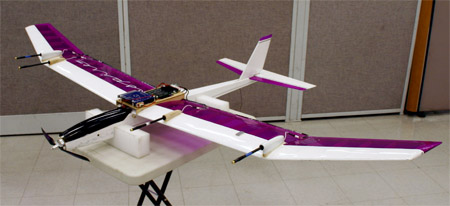
\includegraphics[width=0.75\textwidth]{Figures/Pancas.jpg}
  \caption[PANCAS demonstration aircraft \citep{SARA2012}]{PANCAS demonstration aircraft \citep{SARA2012}}
  \label{fig:pancas}
\end{figure}

\subsection*{Skyward} 
\label{subsection:skyward}

Skyward is an information management platform for commercial UA operators. They provide information to ensure safe flights and in compliance with regulations \citep{Evans2015}. The Drone Airspace Map provides situation awareness with real time area of operations, hazards, restricted zones and temporary flight restrictions, as is shown in figure \ref{fig:skyward}. The platform also allows the creation of flight plans and flight logs, which can then generate the required reports \citep{Skyward2015}.

\begin{figure}[!htb]
  \centering
  \includegraphics[width=0.90\textwidth]{Figures/skyward.png}
  \caption[Skyward example flight area map \citep{Skyward2015}]{Skyward example flight area map \citep{Skyward2015}}
  \label{fig:skyward}
\end{figure}

%\subsection*{Lockheed Martin's Flight Service Pilot Web} 
%\label{subsection:lockheedweb}
%Lockheed Martin's Flight Service Pilot Web \citep{Gibson2015}

\subsection*{AVEO's AECAS100}
\label{subsection:aecas}
The AVEO Collision Avoidance System 100 (AECAS100) is an electronic unit that receives sensor data and steering command from the autopilot or flight management unit (FMU), and provides a correction of the original command to avoid collisions \citep{AEVOGmbH2015}. The sensor data can be transmitted directly to the unit or from a processing unit. Although it can receive data from several types of sensors that use the correct communication protocol, the unit supports direct interface with both RPLidar from RoboPeak and URG-04LX-UG01 from Hokuyo (both laser scanners with maximum range of about 6m).
The AECAS 100 requires obstacle information in two dimensions, which it assumes to be in the horizontal plane, to provide roll and pitch corrections with a frequency of 20 Hz.
Each unit weights 120g and requires between 4.5 and 5.5V and 2.0A of power through a 2.1mm barrel connector, as can be seen in figure \ref{fig:aecas}.

\begin{figure}[!htb]
  \centering
  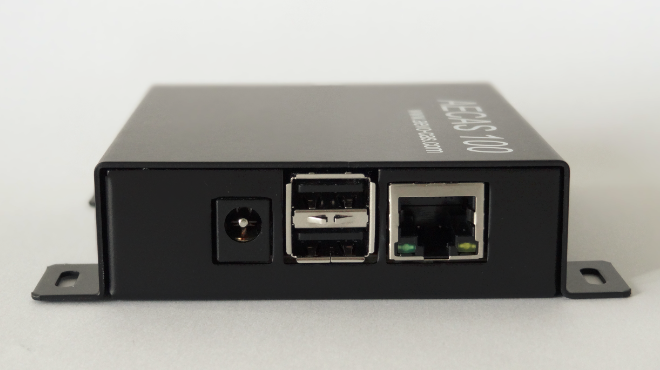
\includegraphics[width=0.6\textwidth]{Figures/aecas100.png}
  \caption[AECAS 100 unit \citep{AEVOGmbH2015a}]{AECAS 100 unit \citep{AEVOGmbH2015a}}
  \label{fig:aecas}
\end{figure}

\subsection*{DJI's guidance} 
\label{subsection:dji}
DJI's guidance is a sensor-based navigation aid \citep{DJI2015}. It uses data from several ultrasonic and image sensors to help avoid obstacles and perform hover by transmitting velocity, position and obstacle clearance to the autopilot.\\
With a weight of 279 g, it requires an input voltage between 11.1 V and 25 V, and consumes a maximum of 12 W. During operation, it requires good lighting and texture-rich surfaces with clear patterns and it is able to measure velocity until 16 m/s with an accuracy of 0.04 m/s. The sensors have a minimum effective range of 0.20 m and maximum of 20 m \citep{DJI2015}.

\begin{figure}[!htb]
  \centering
  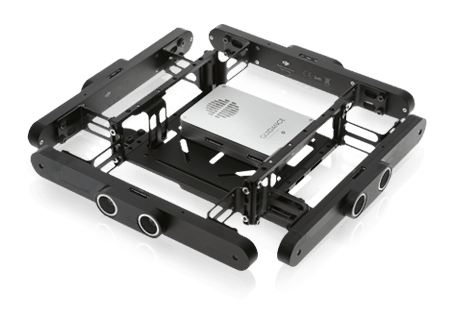
\includegraphics[width=0.6\textwidth]{Figures/guidance.png}
  \caption[DJI Guidance \citep{DJI2015a}]{DJI Guidance \citep{DJI2015a}}
  \label{fig:guidance}
\end{figure}

\subsection*{Unilight} 
\label{subsection:unilight}
Unilight is an Austrian company that manufactures small aircraft lighting. 
All lights are equipped with high performance LEDs to lower consumption and increase visibility.
To enable different behaviors for different types of lights, several controllers are also available which can be programmed according to the specific needs. Controllers range from a simple 1 channel controller, which costs \euro{24.90} and weights approximately 1.5 g without wires, to a USB programmable 8 channel controller, which costs \euro{74.90} and weights 18 g without cables \citep{Rockstroh2014}. 
The available lighting systems cover all the required aircraft lights, such as navigation lights (figure \ref{fig:unilight}) and anti-collision flashers. 
All the available controllers and lights can be directly connected to a 2S battery and come with a resistor that can be added to enable 3S batteries \citep{Mchale2015}.

\begin{figure}[!htb]
  \centering
  \includegraphics[width=0.60\textwidth]{Figures/unilight.png}
  \caption[Unilight navigation light \citep{Rockstroh2014}]{Unilight navigation light \citep{Rockstroh2014}}
  \label{fig:unilight}
\end{figure}

